\def\linkdethi{} %Đường link cần dẫn tới
\anmaQR
%%%%%%%%%%%%%%%%%%%%%%%%
\def\toanlop{12}
\def\thoigian{90}
\def\namhoc{2025 - 2026}
\begin{dethi}
	{Bộ GD\&ĐT}
	{VTED ft KING EDU}
	{TDMZZ04}
	{Đề thi thử THPTQG 2026}
\end{dethi}
\caulc
\Opensolutionfile{ans}[ans/ansTN-Dung]
%%%=============EX_1=============%%%
\begin{ex}%[1D2N2-4]%[TDMZZ03]%[Mui Doan]
	Cho cấp số cộng $(u_n)$ có $u_1=2$ và $d=5$. Giá trị của $u_3$ bằng
	\choice
	{$17$}
	{\True $12$}
	{$18$}
	{$50$}
	\loigiai{
		Ta có $u_3=u_1+2d=2+2\cdot 5=12$.
	}
\end{ex}
%%%=============================%%%

%%%=============EX_2=============%%%
\begin{ex}%[1D6H4-2]%[TDMZZ04]%[Huỳnh Trí Thiện]
	Nghiệm của phương trình $2^{x+3} = 16$ là
	\choice
	{\True $x = 1$}
	{$x = 4$}
	{$x = 5$}
	{$x = 2$}
	\loigiai{
		Ta có
		\[ 2^{x+3} = 16 \Leftrightarrow 2^{x+3} = 2^4 \Leftrightarrow x + 3 = 4 \Leftrightarrow x = 1. \]
		Vậy phương trình đã cho có nghiệm là $x=1$.
	}
\end{ex}
%%%=============================%%%

%%%=============EX_3=============%%%
\begin{ex}%[1D6H4-3]%[TDMZZ04]%[Chu Hà]
	Tập nghiệm của bất phương trình $\log\left(x^2-15x\right)<2$ là
	\choice
	{$(-5;20)$}
	{$(15;20)$}
	{\True $(-5;0)\cup(15;20)$}
	{$(-5;0)$}
	\loigiai{
		Điều kiện xác định $x^2-15x>0 \Leftrightarrow x\in(-\infty;0)\cup(15;+\infty)$.\\
		Ta có
		\begin{eqnarray*}
			&&\log\left(x^2-15x\right)<2 \\
			&\Leftrightarrow& x^2-15x-100<0\\
			&\Leftrightarrow& (x+5)(x-20)<0\\
			&\Leftrightarrow& -5<x<20.
		\end{eqnarray*}
		Kết hợp điều kiện, ta được tập nghiệm $x\in(-5;0)\cup(15;20)$.
	}
\end{ex}
%%%=============================%%%

%%%=============EX_4=============%%%
\begin{ex}%[1H8N2-3]%[TDMZZ04]%[Nguyễn Tấn Linh]
	Cho hình chóp đều $S. ABCD$ có tâm của đáy là $O$. Đáp án cho nhận xét sai là
	\choice
	{$SO \perp (ABCD)$}
	{$BD \perp SA$}
	{$AC \perp SD$}
	{\True $AB \perp SC$}
	\loigiai{
		\begin{center}
			\begin{tikzpicture}[line join=round,line cap=round,font=\footnotesize,scale=1]
				\coordinate (B) at (0,0);
				\coordinate (C) at (4,0);
				\coordinate (A) at (1.5,1.2);
				\coordinate (D) at ($(C)-(B)+(A)$);
				\coordinate (O) at ($(A)!.5!(C)$);
				\coordinate (S) at ($(O)+(90:3.5)$);
				
				\draw (S)--(B)--(C)--(D)--cycle (S)--(C);
				\draw[dashed] (S)--(A)--(B) (A)--(D) (A)--(C) (B)--(D) (S)--(O);
				
				\foreach \diem/\goc in {A/90,B/180,C/-90,D/0,S/90,O/-90} \fill[black](\diem) circle (1pt) ($(\diem)+(\goc:3mm)$) node{$\diem$};
			\end{tikzpicture}
		\end{center}
		Vì $S. ABCD$ là hình chóp đều có tâm đáy là $O$ nên $SO \perp (ABCD)$.\\
		Vì đáy $ABCD$ là hình vuông nên $BD \perp AC$.\\
		Lại có $SO \perp (ABCD) \Rightarrow SO \perp BD$.\\
		Từ đó suy ra $BD \perp (SAC) \Rightarrow BD \perp SA$.\\
		Chứng minh tương tự, ta có $AC \perp BD$ và $AC \perp SO$ nên $AC \perp (SBD) \Rightarrow AC \perp SD$.\\
		Vậy nhận xét sai là $AB \perp SC$.
	}
\end{ex}
%%%=============================%%%

%%%=============EX_5=============%%%
\begin{ex}%[2D1N2-1]%[TDMZZ04]%[Phạm Hải Dương]
	Hàm số $y = x^3 - 24x^2$ đạt cực tiểu tại điểm
	\choice
	{\True $x = 16$}
	{$x = 0$}
	{$y = 16$}
	{$x = -16$}
	\loigiai{
		Tập xác định $\mathscr{D}=\mathbb{R}$.\\
		Ta có $y'=3x^2-48x$.\\
		$y'=0\Leftrightarrow 3x^2-48x=0 \Leftrightarrow 3x(x-16)=0\Leftrightarrow \hoac{&x=0\\&x=16.}$\\
		Ta có $y''=6x-48$.\\
		Với $x=0\Rightarrow y''(0)=-48<0$, hàm số đạt cực đại tại $x=0$.\\
		Với $x=16\Rightarrow y''(16)=48>0$, hàm số đạt cực tiểu tại $x=16$.\\
		Vậy hàm số đạt cực tiểu tại điểm $x=16$.
	}
\end{ex}
%%%=============================%%%

%%%=============EX_6=============%%%
\begin{ex}%[1D5H1-3]%[TDMZZ04]%[Nguyễn Sơn Thành]
	Cho hai mẫu số liệu ghép nhóm $M_1$, $M_2$ với bảng tần số ghép nhóm như sau
	\begin{center}
		Nhóm $M_1$
		\begin{tabular}{|c|c|c|c|c|c|c|}
			\hline
			Nhóm & $\left[5;7\right)$ &$\left[7;9\right)$ &$\left[9;11\right)$ &$\left[11;13\right)$ &$\left[13;15\right)$ &$\left[15;17\right)$ \\
			\hline
			Tần số $M_1$ & $3$ & $5$ & $6$ & $4$ & $6$ & $4$ \\
			\hline
		\end{tabular}
	\end{center}
	
	\begin{center}
		Nhóm $M_2$
		\begin{tabular}{|c|c|c|c|c|c|c|}
			\hline
			Nhóm & $\left[5;7\right)$ &$\left[7;9\right)$ &$\left[9;11\right)$ &$\left[11;13\right)$ &$\left[13;15\right)$ &$\left[15;17\right)$ \\
			\hline
			Tần số $M_2$ & $6$ & $10$ & $12$ & $8$ & $12$ & $10$ \\
			\hline
		\end{tabular}
	\end{center}
	Gọi $\overline{x}_1$, $\overline{x}_2$ lần lượt là số trung bình cộng của hai mẫu số liệu $M_1$, $M_2$. Đáp án so sánh \textbf{đúng} là
	\choice
	{$\overline{x}_1=\overline{x}_2$}
	{\True $\overline{x}_1<\overline{x}_2$}
	{$\overline{x}_1>2\overline{x}_2$}
	{$\overline{x}_1=2\overline{x}_1$}
	\loigiai{
		Ta có
		\begin{itemize}
			\item $\overline{x}_1=\dfrac{6 \cdot 3+8\cdot5 + 10\cdot6+ 12\cdot4+14\cdot6+16\cdot4}{3+5+6+4+6+4}=\dfrac{314}{28}=\dfrac{157}{14}\approx 11{,}21$.
			\item $\overline{x}_2=\dfrac{6 \cdot 6+8\cdot 10 + 10\cdot 12+ 12\cdot 8+14\cdot 12+16\cdot 10}{6+10+12+8+12+10}=\dfrac{660}{58}=\dfrac{330}{29}\approx 11{,}38$.
		\end{itemize}
		Vậy $\overline{x}_1<\overline{x}_2$.
	}
\end{ex}
%%%=============================%%%

%%%=============EX_7=============%%%
\begin{ex}%[2H2N1-2]%[TDMZZ04]%[Bồ Văn Hậu]
	\immini[thm]{Cho hình hộp $ABCD. A'B'C'D'$. Khẳng định nào sau đây là \textbf{đúng}?
		\choice
		{$\overrightarrow{AC}+\overrightarrow{CB'}+\overrightarrow{B'B}=\overrightarrow{AB'}$}
		{$\overrightarrow{AA'}+\overrightarrow{CC'}+\overrightarrow{BB'}=\overrightarrow{AB'}$}
		{\True $\overrightarrow{AC}+\overrightarrow{DD'}+\overrightarrow{C'B'}=\overrightarrow{AB'}$}
		{$\overrightarrow{AB'}+\overrightarrow{B'B}+\overrightarrow{CB'}=\overrightarrow{AB'}$}
	}{
		\begin{tikzpicture}[line cap=round, line join=round, font=\footnotesize, >=stealth, scale=0.6]
			\path 
			(0,0) coordinate (A)
			(5,0) coordinate (D)
			(-2,-2) coordinate (B)
			($(D) - (A) + (B)$) coordinate (C)
			($(A) + (0.5,3)$) coordinate (A')
			($(B) + (0.5,3)$) coordinate (B')
			($(C) + (0.5,3)$) coordinate (C')
			($(D) + (0.5,3)$) coordinate (D')
			;
			\draw[dashed] (A')--(A) (B)--(A)--(D);
			\draw (A')--(B')--(C')--(D')--cycle (D')--(D)--(C) (B')--(B)--(C)--(C')--cycle;
			\foreach \i/\r in {A/150, B/-135, C/-45, D/0, A'/105, B'/180, C'/-45, D'/45}{
				\filldraw[black] (\i) circle (1pt);
				\node at ($(\i) + (\r:4mm)$) {$\i$};
			}
	\end{tikzpicture}}
	\loigiai{
		Ta có $ABCD. A'B'C'D'$ là hình hộp nên $\overrightarrow{DD'}=\overrightarrow{CC'}$, suy ra
		\[ \overrightarrow{AC}+\overrightarrow{DD'}+\overrightarrow{C'B'}=\overrightarrow{AC}+\overrightarrow{CC'}+\overrightarrow{C'B'}=\overrightarrow{AB'}. \]
	}
\end{ex}
%%%=============================%%%

%%%=============EX_8=============%%%
\begin{ex}%[2D4N1-3]%[TDMZZ04]%[Lê Phúc]
	Cho $C$ là một hằng số thực thì họ nguyên hàm của hàm số $f(x)=\dfrac{1}{2x}+\sin x$ là
	\choice
	{\True $\dfrac{1}{2}\ln \left|x\right|-\cos x+C$}
	{$\ln \left|x\right|+\cos x+C$}
	{$\ln \left|x\right|-\cos x+C$}
	{$2\ln \left|x\right|-\cos x+C$}
	\loigiai{
		Ta có $\displaystyle\int \left(\dfrac{1}{2x}+\sin x\right) \mathrm{\,d}x = \dfrac{1}{2}\ln \left|x\right|-\cos x+C$.
	}
\end{ex}
%%%=============================%%%

%%%=============EX_9=============%%%
\begin{ex}%[2H2N2-2]%[TDMZZ04]%[Trần Văn Thiện]
	Trong không gian $Oxyz$ cho điểm $A(3;2;-4)$. Điểm đối xứng với $A$ qua trục $Ox$ có tọa độ là
	\choice
	{$(3;2;-4)$}
	{$(-3;2;-4)$}
	{\True $(3;-2;4)$}
	{ $(-3;-2;4)$}
	\loigiai{
		\begin{itemize}
			\item Hình chiếu của $A$ lên trục $Ox$ là $H(3;0;0)$.
			\item Điểm $A'$ đối xứng với $A$ qua $Ox$ nhận $H$ làm trung điểm nên $A'(3;-2;4)$.
		\end{itemize}
	}
\end{ex}
%%%=============================%%%

%%%=============EX_10=============%%%
\begin{ex}%[2D4H3-1]%[TDMZZ04]%[Đình Nguyên]
	Diện tích hình phẳng giới hạn bởi các đường $y = x^2 - 2x$, $y = 0$, $x = -1$, $x = 3$ là
	\choice
	{\True $4$}
	{$\dfrac{4}{3}$}
	{$1$}
	{$2$}
	\loigiai{
		Diện tích hình phẳng cần tìm là $S = \displaystyle\int\limits_{-1}^{3} \left|x^2 - 2x\right| \mathrm{\,d}x$.\\
		Xét phương trình $x^2 - 2x = 0 \Leftrightarrow \hoac{&x = 0 \\ &x = 2.}$\\
		Ta có bảng xét dấu của biểu thức $f(x) = x^2 - 2x$ trên đoạn $[-1; 3]$.
		\begin{center}
			
\begin{tikzpicture}[scale=0.8, font=\footnotesize, line join=round, line cap=round, >=stealth]
				\tkzTabInit[nocadre=false, lgt=1.2, espcl=2.5, deltacl=0.6]
				{$x$ /0.6, $f(x)$ /0.6}
				{$-1$, $0$, $2$, $3$}
				\tkzTabLine{, +, 0, -, 0, +, }
			\end{tikzpicture}
		\end{center}
		Khi đó
		\allowdisplaybreaks
		\begin{eqnarray*}
			S &=& \displaystyle\int\limits_{-1}^{0} (x^2 - 2x) \mathrm{\,d}x - \displaystyle\int\limits_{0}^{2} (x^2 - 2x) \mathrm{\,d}x + \displaystyle\int\limits_{2}^{3} (x^2 - 2x) \mathrm{\,d}x \\
			&=& \left. \left( \dfrac{x^3}{3} - x^2 \right) \right|_{-1}^{0} - \left. \left( \dfrac{x^3}{3} - x^2 \right) \right|_{0}^{2} + \left. \left( \dfrac{x^3}{3} - x^2 \right) \right|_{2}^{3}\\
			&=& \dfrac{4}{3} + \dfrac{4}{3} + \dfrac{4}{3} = 4.
		\end{eqnarray*}
		Vậy diện tích hình phẳng là $4$.
	}
\end{ex}
%%%=============================%%%

%%%=============EX_11=============%%%
\begin{ex}%[2D1H4-1]%[TDMZZ04]%[Thêm vào]
	Trong các mệnh đề dưới đây, hỏi có bao nhiêu mệnh đề đúng?
	\begin{enumerate}[1.]
		\item Tiệm cận ngang của một đồ thị $(C)$ luôn không cắt đồ thị $(C)$.
		\item Tiệm cận đứng của một đồ thị $(C)$ có thể có điểm chung với đồ thị $(C)$.
		\item Một đồ thị $(C)$ có tối đa hai đường tiệm cận ngang.
		\item Đồ thị $(C)$ có thể có vô số các đường tiệm cận đứng.
	\end{enumerate}
	\choice
	{\True $3$}
	{$4$}
	{$2$}
	{$1$}
	\loigiai{
		\begin{itemize}
			\item Mệnh đề 1 sai. Đồ thị hàm số có thể cắt đường tiệm cận ngang của nó (ví dụ đồ thị hàm số $y = \dfrac{\sin x}{x}$ cắt TCN $y=0$ tại vô số điểm).
			\item Mệnh đề 2 đúng. Đối với các hàm số cho bởi nhiều công thức, đồ thị hoàn toàn có thể có điểm chung với đường tiệm cận đứng.\\
			Ví dụ: Xét hàm số $y = f(x) = \heva{& \dfrac{1}{x} &&\text{khi } x \neq 0 \\ & 0 &&\text{khi } x = 0.}$ \\
			Ta có $\lim\limits_{x \to 0^+} f(x) = +\infty$ nên đường thẳng $x=0$ là tiệm cận đứng. Tuy nhiên đồ thị hàm số vẫn được xác định tại $x=0$ và đi qua điểm $O(0;0)$ nằm trên chính đường tiệm cận đứng đó.
			\item Mệnh đề 3 đúng. Vì khi xét tiệm cận ngang ta chỉ xét giới hạn của hàm số khi $x \to +\infty$ và $x \to -\infty$, nên có tối đa $2$ đường tiệm cận ngang.
			\item Mệnh đề 4 đúng. Đồ thị hàm số có thể có vô số đường tiệm cận đứng, ví dụ đồ thị hàm số $y = \tan x$ có vô số đường tiệm cận đứng $x = \dfrac{\pi}{2} + k\pi$ ($k \in \mathbb{Z}$).
		\end{itemize}
		Vậy có $3$ mệnh đề đúng.
	}
\end{ex}
%%%=============================%%%

%%%=============EX_12=============%%%
\begin{ex}%[2H5N2-3]%[TDMZZ04]%[Nguyễn Trí Minh Tuấn]
	Trong không gian $Oxyz$, phương trình chính tắc của đường thẳng đi qua hai điểm $A(0;2;1)$ và $B(1;-1;3)$ là
	\choice
	{$\dfrac{x}{1}=\dfrac{y+2}{-3}=\dfrac{z+1}{2}$}
	{$\dfrac{x}{1}=\dfrac{y-2}{3}=\dfrac{z-1}{-2}$}
	{$\dfrac{x-1}{1}=\dfrac{y+1}{-3}=\dfrac{z-3}{-2}$}
	{\True $\dfrac{x+1}{-1}=\dfrac{y-5}{3}=\dfrac{z+1}{-2}$}
	\loigiai{
		Ta có, một vectơ chỉ phương của đường thẳng đi qua hai điểm $A$ và $B$ là
		\[ \overrightarrow{AB}=(1-0; -1-2; 3-1)=(1;-3;2). \]
		Do đó, đáp án chỉ có thể là $\dfrac{x}{1}=\dfrac{y+2}{-3}=\dfrac{z+1}{2}$ hoặc $\dfrac{x+1}{-1}=\dfrac{y-5}{3}=\dfrac{z+1}{-2}$.\\
		Thế tọa độ điểm $A$ vào hai phương trình trên, ta thấy phương trình thỏa mãn là $\dfrac{x+1}{-1}=\dfrac{y-5}{3}=\dfrac{z+1}{-2}$.
	}
\end{ex}
%%%=============================%%%
\Closesolutionfile{ans}
\cauds
\Opensolutionfile{ans}[ans/ansTN-DungSai]
%%%=============EX_13=============%%%
\begin{ex}%[2D4H2-4]%[TDMZZ03]%[Văn Minh Thoại]
	Cho giá trị trung bình của hàm số $f(x)$ trên đoạn $[a;b]$ là $\overline{f([a;b])}=\dfrac{1}{b-a}\displaystyle\int\limits_a^b f(x)\mathrm{\,d}x$, với $f(x)$ liên tục trên $[a;b]$.
	\choiceTF
	{\True Nếu $f(x)=x^2-3x$ thì $\overline{f([1;2])}=-\dfrac{13}{6}$}
	{Nếu $f(x)=\mathrm{e}^x+\sin x$ thì $\overline{f([0;\pi])}=\dfrac{5\pi}{3}$}
	{\True $\overline{f([1;2])}+\overline{f([2;3])}=2\overline{f([1;3])}$}
	{Nếu $\overline{f([1;2])}=3$, $\overline{f([2;4])}=4$ thì $\overline{f([1;4])}=7$}
	\loigiai{
		\begin{itemchoice}
			\itemch Ta có
			\begin{eqnarray*}
				\overline{f([1;2])}&=&\dfrac{1}{2-1}\displaystyle\int\limits_1^2\left(x^2-3x\right)\mathrm{\,d}x\\
				&=&\left.\left(\dfrac{x^3}{3}-\dfrac{3x^2}{2}\right)\right|_1^2\\
				&=&\left(\dfrac{8}{3}-6\right)-\left(\dfrac{1}{3}-\dfrac{3}{2}\right)\\
				&=&-\dfrac{13}{6}.
			\end{eqnarray*}
			\itemch Ta có
			\begin{eqnarray*}
				\overline{f([0;\pi])}&=&\dfrac{1}{\pi-0}\displaystyle\int\limits_0^\pi\left(\mathrm{e}^x+\sin x\right)\mathrm{\,d}x\\
				&=&\dfrac{1}{\pi}\left.\left(\mathrm{e}^x-\cos x\right)\right|_0^\pi\\
				&=&\dfrac{1}{\pi}\left[\left(\mathrm{e}^\pi-(-1)\right)-(1-1)\right]\\
				&=&\dfrac{\mathrm{e}^\pi+1}{\pi}\neq\dfrac{5\pi}{3}.
			\end{eqnarray*}
			\itemch Ta có
			\begin{eqnarray*}
				\overline{f([1;2])}+\overline{f([2;3])}&=&\dfrac{1}{2-1}\displaystyle\int\limits_1^2 f(x)\mathrm{\,d}x+\dfrac{1}{3-2}\displaystyle\int\limits_2^3 f(x)\mathrm{\,d}x\\
				&=&\displaystyle\int\limits_1^2 f(x)\mathrm{\,d}x+\displaystyle\int\limits_2^3 f(x)\mathrm{\,d}x\\
				&=&\displaystyle\int\limits_1^3 f(x)\mathrm{\,d}x.
			\end{eqnarray*}
			Mặt khác, $2\overline{f([1;3])}=2\cdot\dfrac{1}{3-1}\displaystyle\int\limits_1^3 f(x)\mathrm{\,d}x=\displaystyle\int\limits_1^3 f(x)\mathrm{\,d}x$.\\
			Do đó $\overline{f([1;2])}+\overline{f([2;3])}=2\overline{f([1;3])}$.
			\itemch Theo giả thiết, $\overline{f([1;2])}=3 \Rightarrow \dfrac{1}{2-1}\displaystyle\int\limits_1^2 f(x)\mathrm{\,d}x=3 \Rightarrow \displaystyle\int\limits_1^2 f(x)\mathrm{\,d}x=3$.\\
			Và $\overline{f([2;4])}=4 \Rightarrow \dfrac{1}{4-2}\displaystyle\int\limits_2^4 f(x)\mathrm{\,d}x=4 \Rightarrow \displaystyle\int\limits_2^4 f(x)\mathrm{\,d}x=8$.\\
			Suy ra $\overline{f([1;4])}=\dfrac{1}{4-1}\displaystyle\int\limits_1^4 f(x)\mathrm{\,d}x=\dfrac{1}{3}\left(\displaystyle\int\limits_1^2 f(x)\mathrm{\,d}x+\displaystyle\int\limits_2^4 f(x)\mathrm{\,d}x\right)=\dfrac{1}{3}\cdot (3+8)=\dfrac{11}{3}\neq 7$.
		\end{itemchoice}
	}
\end{ex}
%%%=============================%%%

%%%=============EX_14=============%%%
\begin{ex}%[2D1V5-7]%[TDMZZ04]%[Dương Công Tạo]
	Trong mặt phẳng $Oxy$, cho hàm số $y = f(x) = 3x^2 - 4$. Gọi $F(x)$ một nguyên hàm của hàm số $f(x)$ trên $\mathbb{R}$. Biết đồ thị $(C)$ của hàm số $y = \dfrac{1}{F(x)}$ có tiệm cận đứng là trục tung $Oy$.
	\choiceTF
	{\True $(C)$ có tất cả $4$ đường tiệm cận}
	{Khoảng cách hai điểm cực trị của đồ thị hàm số $y = F(x)$ bằng $6\sqrt{3}$}
	{\True Diện tích hình phẳng giới hạn bởi đồ thị hàm số $y = F(x)$ với $Ox$ bằng $8$}
	{Có tất cả $66$ đường thẳng cắt đồ thị của hàm số $y = \dfrac{F(x)}{x^2 - 4x}$ tại hai điểm phân biệt là những điểm có toạ độ nguyên}
	\loigiai{
		\begin{itemchoice}
			\itemch Ta có $F(x)=\displaystyle\int\left(3x^2 - 4\right)\mathrm{\,d}x=x^3-4x+C$.\\
			Vì đồ thị $(C)$ của hàm số $y = \dfrac{1}{F(x)}$ có tiệm cận đứng là trục tung $Oy$ nên $x=0$ là nghiệm của phương trình $F(x)=0 \Rightarrow C=0$.\\
			Suy ra $F(x)=x^3-4x$.\\
			Khi đó, hàm số $y = \dfrac{1}{x^3-4x}$ có tập xác định $\mathscr{D}=\mathbb{R}\setminus\left\{0;\pm 2\right\}$.\\
			Ta có \begin{itemize}
				\item $\lim\limits_{x\to 0^-}y=+\infty$, $\lim\limits_{x\to 2^-}y=-\infty$ và $\lim\limits_{x\to -2^-}y=-\infty$.\\ Suy ra đồ thị $(C)$ của hàm số có $3$ đường tiệm cận đứng là $x=0$, $x=2$ và $x=-2$.
				\item $\lim\limits_{x\to \pm \infty}y=0$ suy ra đồ thị $(C)$ của hàm số có $1$ đường tiệm cận ngang là $y=0$.
			\end{itemize}
			Vậy, $(C)$ có tất cả $4$ đường tiệm cận.
			\itemch Xét hàm số $F(x)=x^3-4x$.\\
			Ta có $F'(x)= 3x^2-4$, $F'(x)= 0\Leftrightarrow 3x^2-4=0\Leftrightarrow x=\pm\dfrac{2}{\sqrt{3}}$.\\
			Bảng biến thiên
			\begin{center}
				
\begin{tikzpicture}[>=stealth]
					\tkzTabInit[nocadre=false,lgt=1.5,espcl=2,deltacl=0.6]{$x$/1 ,$F'(x)$/.7,$F(x)$/2}
					{$-\infty$ , $-\dfrac{2}{\sqrt{3}}$ , $\dfrac{2}{\sqrt{3}}$ , $+\infty$}
					\tkzTabLine{ , + , 0 , - , 0 , + ,  }
					\tkzTabVar{-/$-\infty$ , +/$\dfrac{16}{3\sqrt{3}}$ , -/$-\dfrac{16}{3\sqrt{3}}$ ,+/$+\infty$}
				\end{tikzpicture}
			\end{center}
			Dựa vào bảng biến thiên, ta thấy đồ thị đạt cực đại tại điểm $A\left(-\dfrac{2}{\sqrt{3}};\dfrac{16}{3\sqrt{3}}\right)$, cực tiểu tại điểm $B\left(\dfrac{2}{\sqrt{3}};-\dfrac{16}{3\sqrt{3}}\right)$.\\
			Khi đó, độ dài đoạn $AB=\sqrt{\left(\dfrac{4}{\sqrt{3}}\right)^2 + \left(-\dfrac{32}{3\sqrt{3}}\right)^2} = \dfrac{4\sqrt{91}}{9} \neq 6\sqrt{3}$.
			\itemch Phương trình hoành độ giao điểm $x^3-4x=0\Leftrightarrow\hoac{&x=0\\&x=\pm 2.}$\\
			Khi đó, diện tích hình phẳng giới hạn bởi đồ thị hàm số $y = F(x)$ với $Ox$ là
			\[S=\displaystyle\int\limits_{-2}^2\left|x^3 - 4x\right|\mathrm{\,d}x = 2\displaystyle\int\limits_{0}^2 (4x - x^3)\mathrm{\,d}x = 2\left.\left(2x^2 - \dfrac{x^4}{4}\right)\right|_0^2 = 8.\]
			\itemch Với $F(x)=x^3 - 4x$, hàm số $y = \dfrac{F(x)}{x^2 - 4x}$ trở thành $y=\dfrac{x(x^2-4)}{x(x-4)} = \dfrac{x^2-4}{x-4}=x+4+\dfrac{12}{x-4}$ với điều kiện $x \notin \{0; 4\}$.\quad(1)\\
			Gọi $M(x;y)$ là những điểm trên đồ thị hàm số $(1)$ có toạ độ là những số nguyên.\\
			Ta có $x\in\mathbb{Z} \setminus \{0; 4\}$, $y \in \mathbb{Z} \Leftrightarrow x+4+\dfrac{12}{x-4}\in\mathbb{Z}\Rightarrow (x-4)\in\text{Ư}(12)\Leftrightarrow (x-4)\in\left\{\pm 1;\pm 2;\pm 3;\pm 4;\pm 6;\pm 12\right\}$.\\
			Vì $x \neq 0$ nên $x-4 \neq -4$. Do đó ta loại trường hợp $(x-4) = -4$.\\
			Suy ra, trên đồ thị hàm số $(1)$ chỉ có $12 - 1 = 11$ điểm có toạ độ là số nguyên.\\
			Ta chứng minh trong $11$ điểm trên không có ba điểm nào thẳng hàng. Thật vậy, đặt $d=x-4$, khi đó $d\in\text{Ư}(12)$ và $d\neq -4$, đồng thời
			\[
			x=d+4,\quad y=d+8+\dfrac{12}{d}.
			\]
			Xét hai điểm nguyên phân biệt ứng với $d=a$ và $d=b$ với $a\neq b$. Hệ số góc của đường thẳng đi qua hai điểm đó là
			\[
			k_{ab}=\dfrac{\left(b+8+\dfrac{12}{b}\right)-\left(a+8+\dfrac{12}{a}\right)}{(b+4)-(a+4)}
			=1-\dfrac{12}{ab}.
			\]
			Nếu ba điểm nguyên phân biệt ứng với $d=a$, $d=b$, $d=c$ thẳng hàng thì
			\[
			k_{ab}=k_{ac}
			\Leftrightarrow 1-\dfrac{12}{ab}=1-\dfrac{12}{ac}
			\Leftrightarrow b=c,
			\]
			mâu thuẫn với giả thiết ba điểm phân biệt. Vậy không có ba điểm nguyên nào thẳng hàng.\\
			Do đó, số đường thẳng cắt đồ thị hàm số $(1)$ tại hai điểm có toạ độ nguyên là $\mathrm{C}_{11}^2=55$ đường thẳng. Mệnh đề sai.
		\end{itemchoice}
	}
\end{ex}

%%%=============================%%%

%%%=============EX_15=============%%%
\begin{ex}%[2H5V3-4]%[TDM31]
	Trong không gian với hệ tọa độ $Oxyz$ (đơn vị trên mỗi trục là kilômét), một trạm thu phát sóng điện thoại di động được đặt ở vị trí $I(-5;1;6)$. Biết rằng trạm thu phát sóng đó được thiết kế với bán kính phủ sóng là $4$ km.
	\choiceTF
	{\True Mặt cầu mô tả ranh giới phần bên ngoài và bên trong vùng phủ sóng trong không gian có phương trình là $(x+5)^2 + (y-1)^2 + (z-6)^2 = 16$}
	{Nếu người dùng điện thoại ở điểm $A(0;2;9)$ thì có thể sử dụng dịch vụ này}
	{\True Người dùng điện thoại đang ở $A$, muốn sử dụng được dịch vụ phải di chuyển một đoạn ngắn nhất bằng $1{,}92$ km \textit{(làm tròn kết quả đến hàng phần trăm)}}
	{Một người đang ở vị trí $B(-3;1;4)$ mà muốn thoát khỏi vùng phủ sóng thì phải di chuyển một đoạn ngắn nhất bằng $1{,}71$ km}
	\loigiai{
		Trạm phát sóng tại $I(-5;1;6)$ có bán kính phủ sóng $R = 4$ km.\\
		Vùng phủ sóng là một khối cầu tâm $I$, bán kính $R=4$.
		\begin{center}
			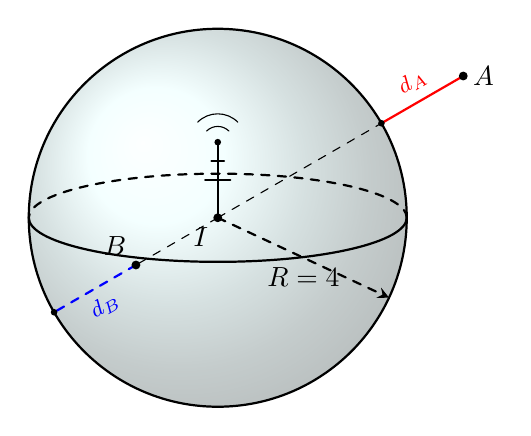
\begin{tikzpicture}[scale=0.8, line join=round, line cap=round, >=stealth]
				\def\R{3} 
				
				% Khối cầu 3D trong suốt
				\shade[ball color=cyan!15, opacity=0.4] (0,0) circle (\R);
				\draw[thick] (0,0) circle (\R);
				
				% Đường xích đạo tạo cảm giác 3D
				\draw[dashed, thick] (\R,0) arc (0:180:\R cm and 0.7cm);
				\draw[thick] (\R,0) arc (0:-180:\R cm and 0.7cm);
				
				% Tâm I
				\coordinate (I) at (0,0);
				\fill (I) circle (2pt) node[below left] {$I$};
				
				% Trạm phát sóng tại I
				\draw[thick, line cap=butt] (0,0) -- (0,1.2);
				\draw[thick] (-0.2,0.6) -- (0.2,0.6);
				\draw[thick] (-0.1,0.9) -- (0.1,0.9);
				\fill (0,1.2) circle (1.5pt);
				\draw (0,1.2) ++(45:0.25) arc (45:135:0.25);
				\draw (0,1.2) ++(45:0.45) arc (45:135:0.45);
				
				% Bán kính R
				\draw[->,dashed, thick] (I) -- (-25:\R) node[midway, below] {$R=4$};
				
				% Điểm A (Nằm ngoài mặt cầu)
				\coordinate (A) at (30:4.5);
				\coordinate (M) at (30:\R); 
				\draw[dashed] (I) -- (M);
				\draw[thick, red] (M) -- (A) node[midway, above, sloped] {\footnotesize $d_A$};
				\fill (M) circle (1.5pt);
				\fill (A) circle (2pt) node[right] {$A$};
				
				% Điểm B (Nằm trong mặt cầu)
				\coordinate (B) at (210:1.5);
				\coordinate (N) at (210:\R); 
				\draw[dashed] (I) -- (B);
				\draw[thick, dashed, blue] (B) -- (N) node[midway, below, sloped] {\footnotesize $d_B$};
				\fill (B) circle (2pt) node[above left] {$B$};
				\fill (N) circle (1.5pt);
			\end{tikzpicture}
		\end{center}
		\begin{itemchoice}
			\itemch Phương trình mặt cầu ranh giới là $(x+5)^2 + (y-1)^2 + (z-6)^2 = 4^2 = 16$.
			\itemch Xét điểm $A(0;2;9)$. Khoảng cách từ $A$ đến trạm phát $I$ là
			\[ IA = \sqrt{(0-(-5))^2 + (2-1)^2 + (9-6)^2} = \sqrt{5^2 + 1^2 + 3^2} = \sqrt{35} \approx 5{,}92 \text{ km}. \]
			Vì $IA > R$ ($5{,}92 > 4$) nên người dùng ở $A$ nằm ngoài vùng phủ sóng, không thể sử dụng dịch vụ.
			\itemch Để người ở $A$ sử dụng được dịch vụ, người đó phải di chuyển vào trong mặt cầu. Khoảng cách ngắn nhất là
			\[ \mathrm{d}_{\min} = IA - R = \sqrt{35} - 4 \approx 5{,}916 - 4 = 1{,}916 \approx 1{,}92 \text{ km}. \]
			\itemch Xét điểm $B(-3;1;4)$. Khoảng cách từ $B$ đến trạm phát $I$ là
			\[ IB = \sqrt{(-3-(-5))^2 + (1-1)^2 + (4-6)^2} = \sqrt{2^2 + 0^2 + (-2)^2} = \sqrt{8} \approx 2{,}83 \text{ km}. \]
			Vì $IB < R$ ($2{,}83 < 4$) nên người ở $B$ đang ở trong vùng phủ sóng.
			Để thoát khỏi vùng phủ sóng, người đó phải di chuyển ra ngoài mặt cầu, đoạn ngắn nhất là
			\[ \mathrm{d}_{\min} = R - IB = 4 - \sqrt{8} \approx 4 - 2{,}828 = 1{,}172 \approx 1{,}17 \text{ km}. \]
		\end{itemchoice}
	}
\end{ex}
%%%=============================%%%

%%%=============EX_16=============%%%
\begin{ex}%[2D6V2-4]%[TDMZZ04]%[Vũ Hồng Toàn]
	Cho hai cờ thủ X và Y thi đấu với nhau. Chỉ số tổng lực ban đầu của X và Y lần lượt là $40$ và $60$. Biết rằng xác suất chiến thắng của mỗi cờ thủ trong một trận đấu bằng tỉ lệ chỉ số tổng lực của cờ thủ đó chia cho tổng chỉ số tổng lực của hai cờ thủ ngay trước trận đấu đó. Với giả thiết sau mỗi trận mà X thắng thì chỉ số tổng lực của X sẽ tăng $20\%$ so với ngay trước đó và nếu thua thì chỉ số tổng lực giảm $25\%$ so với ngay trước đó, còn cờ thủ Y thì ổn định hơn sau mỗi trận mà Y thắng chỉ số tổng lực tăng $14\%$ và thua thì giảm $10\%$ so với ngay trước đó. Gọi $A$ là biến cố trận đầu tiên X thắng, $B$ là biến cố trận thứ hai X thắng.
	\choiceTF
	{\True $\mathrm{P}(A)=0{,}4$}
	{$\mathrm{P}(B\mid A)=\dfrac{9}{17}$}
	{\True $\mathrm{P}(B)=0{,}37$ \textit{(làm tròn kết quả đến hàng phần trăm)}}
	{\True $\mathrm{P}(A\mid B)=0{,}51$ \textit{(làm tròn kết quả đến hàng phần trăm)}}
	\loigiai{
		\begin{itemchoice}
			\itemch Ta có $n(A)=40$ và $n(B)=60$. Suy ra tổng chỉ số ban đầu là $n(\Omega)=n(A)+n(B)=40+60=100$.\\
			Vậy $\mathrm{P}(A)=\dfrac{n(A)}{n(\Omega)}=\dfrac{40}{100}=0{,}4$.
			\itemch Nếu X thắng trận đầu tiên (biến cố $A$ xảy ra):\\
			Chỉ số tổng lực của X sau trận đầu tiên là $X_1 = n(A) \cdot (1 + 20\%) = 48$.\\
			Chỉ số tổng lực của Y sau trận đầu tiên là $Y_1 = n(B) \cdot (1 - 10\%) = 54$.\\
			Tổng chỉ số tổng lực sau trận đầu tiên là $S_1 = X_1 + Y_1 = 48 + 54 = 102$.\\
			Xác suất X thắng trận thứ hai trong trường hợp này là $\mathrm{P}(B\mid A) = \dfrac{X_1}{S_1} = \dfrac{48}{102} = \dfrac{8}{17} \neq \dfrac{9}{17}$.
			\itemch Xét trường hợp $\overline{A}$ (X thua trận đầu tiên): $\mathrm{P}\left(\overline{A}\right) = 0{,}6$.\\
			Chỉ số thay đổi:
			\begin{itemize}
				\item $X_2 = 40 \cdot 0{,}75 = 30$.
				\item $Y_2 = 60 \cdot 1{,}14 = 68{,}4$.
				\item Tổng chỉ số mới là $S_2 = 30 + 68{,}4 = 98{,}4$.
				\item Xác suất X thắng trận 2 lúc này là $\mathrm{P}\left(B\mid\overline{A}\right) = \dfrac{30}{98{,}4} = \dfrac{25}{82}$.
			\end{itemize}
			Áp dụng công thức xác suất toàn phần, ta có
			\allowdisplaybreaks
			\begin{eqnarray*}
				\mathrm{P}(B) &=& \mathrm{P}(A) \cdot \mathrm{P}(B\mid A) + \mathrm{P}\left(\overline{A}\right) \cdot \mathrm{P}\left(B\mid\overline{A}\right) \\
				&=& 0{,}4 \cdot \dfrac{8}{17} + 0{,}6 \cdot \dfrac{25}{82} \\
				&\approx& 0{,}37.
			\end{eqnarray*}
			\itemch Sử dụng công thức Bayes:
			\allowdisplaybreaks
			\begin{eqnarray*}
				\mathrm{P}(A\mid B) = \dfrac{\mathrm{P}(A) \cdot \mathrm{P}(B\mid A)}{\mathrm{P}(B)}
				= \dfrac{0{,}4\cdot \dfrac{8}{17}}{0{,}37}\approx 0{,}51.
			\end{eqnarray*}
		\end{itemchoice}
	}
\end{ex}
%%%=============================%%%
\Closesolutionfile{ans}
\caukq
\Opensolutionfile{ans}[ans/ansTN-DienKhuyet]
%%%=============EX_17=============%%%
\begin{ex}%[1D6V4-6]%[TDMZZ04]%[Võ Hiệp]
	\textit{Câu chuyện về mối tình đầu của giới trẻ thì nó rất là thú vị và hấp dẫn, yêu thì nồng nhiệt hết mình mà chia tay thì cũng phũ phàng quyết liệt không kém. Thế nhưng dù có như thế nào thì mối tình đầu cũng rất là khó phai}. \\
	Giả sử có một mối tình đầu giữa hai bạn \textbf{Huỳnh Thanh Nam} và \textbf{Nguyễn Minh Thư} khi còn yêu nhau ta coi như có $100$ điểm tình cảm. Vào một ngày nọ, vì một số lí do hiểu lầm không thể nào giải thích giữa đôi nam nữ này mà dẫn tới họ quyết định chia tay nhau. Ở những ngày sau đó coi như họ gặp nhau mỗi ngày một lần, coi như sau một ngày không gặp nhau thì tình cảm giảm đi $30\%$ so với lúc vừa gặp nhau xong, mỗi lần gặp nhau lại hâm nóng tình cảm và tăng lên $12\%$ so với ngày trước đó. Với giả sử điểm tình cảm nhỏ hơn $10$ thì coi như quên hẳn được nhau và khi gặp sẽ không còn hâm nóng lên được nữa. Hỏi sau tối thiểu bao nhiêu ngày kể từ lúc chia tay thì hai bạn này quên được nhau (\textit{làm tròn kết quả đến hàng đơn vị}).
	\par
	\shortans[0]{9}
	\loigiai{
		Gọi $u_n$ là điểm tình cảm của hai bạn ngay sau lần gặp mặt ở ngày thứ $n$ (với $n \in \mathbb{N}^*$) và $u_0 = 100$.\\
		Sau $1$ ngày không gặp, điểm tình cảm giảm $30\%$, tức là còn lại $70\%$ (nhân với $0{,}7$) so với điểm sau lần gặp trước đó.\\
		Nếu điểm tình cảm lúc này vẫn $\ge 10$, họ gặp nhau và điểm tăng thêm $12\%$, tức là nhân với $1{,}12$.\\
		Khi đó, điểm tình cảm sau lần gặp ở ngày thứ $n$ là
		\[u_n = u_{n-1} \cdot 0{,}7 \cdot 1{,}12 = u_{n-1} \cdot 0{,}784 \Rightarrow u_{n-1} = 100 \cdot (0{,}784)^{n-1}.\]
		Tuy nhiên, điều kiện để hai bạn quên hẳn nhau là điểm tình cảm \textbf{trước khi gặp mặt} nhỏ hơn $10$. \\
		Điểm tình cảm trước khi gặp mặt ở ngày thứ $n$ là $u_{n-1} \cdot 0{,}7$. Ta có bất phương trình:
		\begin{eqnarray*}
			&& u_{n-1} \cdot 0{,}7 < 10 \\
			&\Leftrightarrow& 100 \cdot (0{,}784)^{n-1} \cdot 0{,}7 < 10 \\
			&\Leftrightarrow& (0{,}784)^{n-1} < \dfrac{1}{7} \\
			&\Leftrightarrow& n - 1 > \log_{0{,}784} \left(\dfrac{1}{7}\right) \approx 7{,}996 \\
			&\Leftrightarrow& n > 8{,}996.
		\end{eqnarray*}
		Vì $n$ là số nguyên dương nên ta chọn $n = 9$.\\
		Thử lại: Trước khi gặp nhau ở ngày thứ $9$, điểm tình cảm của hai bạn là $100 \cdot (0{,}784)^8 \cdot 0{,}7 \approx 9{,}991 < 10$ (hai bạn đã quên nhau trước khi kịp hâm nóng).\\
		Vậy sau tối thiểu $9$ ngày thì hai bạn này quên được nhau.
	}
\end{ex}
%%%=============================%%%

%%%=============EX_18=============%%%
\begin{ex}%[2H5V3-4]%[TDMZZ04]%[Lương Pho]
	Ở một xó nhà người ta có gắn một giá đỡ gồm ba thanh cứng tạo thành tam giác $ABC$ như hình vẽ. Đặt một quả cầu phong thuỷ làm bằng đá tự nhiên có bán kính bằng $19$ cm trên giá đỡ $ABC$ sao cho các cạnh của $\triangle ABC$ tiếp xúc với quả cầu phong thuỷ. Để quản lý không gian của ngôi nhà người ta gắn vào hệ trục toạ độ $Oxyz$ với sàn nhà là mặt phẳng $(Oxy)$, đơn vị dài trên mỗi trục tính theo centimet, có toạ độ các điểm $A(20;300;150)$, $B(20;278;150)$, $C(42;300;150)$. Hãy tính độ cao của điểm cao nhất của quả cầu so với sàn nhà theo đơn vị centimet (\textit{làm tròn kết quả đến hàng đơn vị}).
	\par
	\shortans[0]{187}
	\loigiai{
		Ba điểm $A$, $B$, $C$ đều có cao độ $z = 150$, nên mặt phẳng $(ABC)$ song song với mặt sàn $(Oxy)$ và có phương trình $z = 150$.\\
		Quả cầu tiếp xúc với ba cạnh của tam giác $ABC$. \\
		Gọi $I$ là tâm quả cầu, $R=19$ là bán kính quả cầu, và $r$ là bán kính đường tròn nội tiếp $\triangle ABC$.\\
		Ta có $AB = \sqrt{(20-20)^2 + (278-300)^2 + (150-150)^2} = 22$. \\
		$AC = \sqrt{(42-20)^2 + (300-300)^2 + (150-150)^2} = 22$. \\
		$BC = \sqrt{(42-20)^2 + (300-278)^2 + (150-150)^2} = 22\sqrt{2}$. \\
		Suy ra $\triangle ABC$ vuông cân tại $A$.\\
		Bán kính đường tròn nội tiếp $\triangle ABC$ là
		\[ r = \dfrac{S}{p} = \dfrac{\dfrac{1}{2} \cdot 22 \cdot 22}{\dfrac{22+22+22\sqrt{2}}{2}}= 11\left(2-\sqrt{2}\right). \]
		Gọi $h$ là khoảng cách từ tâm quả cầu đến mặt phẳng $(ABC)$.\\
		Vì quả cầu tiếp xúc với các cạnh $\triangle ABC$ nên
		\[ h = \sqrt{R^2 - r^2} = \sqrt{19^2 - \left[11\left(2-\sqrt{2}\right)\right]^2} \approx 17{,}87\,\text{(cm)}. \]
		Độ cao của điểm cao nhất của quả cầu so với sàn nhà là
		\[ H = z_A + h + R = 150 + 17{,}87 + 19 \approx 187\,\text{(cm)}. \]
	}
\end{ex}
%%%=============================%%%

%%%=============EX_19=============%%%
\begin{ex}%[2H2C2-6]%[TDMZZ04]%[Hà Văn Hảo]
	Từ điểm $A$ trên mặt đất hai con bọ rùa I và II bò sát mặt đất theo hai hướng tạo với nhau một góc $50^\circ$, với tốc độ lần lượt là $4$ cm/s và $5$ cm/s, sau đó $20$ giây thì hai con bọ rùa bắt đầu đổi hướng bay lên trên không theo hai hướng vuông góc với các hướng ban đầu của chúng. Do lúc bò ở mặt đất con bọ rùa II bò nhanh quá nên thấm mệt và khi chuyển động trên không tốc độ của nó chỉ bằng một nửa con bọ rùa I. Biết rằng hai con bọ rùa này gặp nhau tại điểm $B$. Hãy xác định độ cao của điểm $B$ so với mặt đất theo đơn vị centimet (\textit{làm tròn kết quả đến hàng phần mười}).
	\par
	\shortans[0]{27,9}
	\loigiai{
		\immini{Gọi $M$, $N$ lần lượt là vị trí của con bọ rùa I và II sau $20$ giây bò trên mặt đất.
			\begin{itemize}
				\item Khoảng cách $AM = 4 \cdot 20 = 80$ cm.
				\item Khoảng cách $AN = 5 \cdot 20 = 100$ cm.
			\end{itemize}
			Gọi $B$ là điểm gặp nhau của hai con bọ rùa trong không gian;\\
			$H$ là hình chiếu của $B$ lên mặt đất.\\
		}{
			\begin{tikzpicture}[scale=0.6, font=\footnotesize, line join=round, line cap=round, >=stealth, declare function={m=4;b=3.5;goc=-135;goc1=-45;h=5;}]
				\path
				(0, 0) coordinate (A)
				(b,0) coordinate (C)
				(goc:m)coordinate (M)
				(goc1:b) coordinate (N)
				($(M)+(C)-(A)$)coordinate (H)
				(H)++(0,h) coordinate (B);
				\draw [->](A)--	($(A)!1.3!(M)$)node[below]{$x$};
				\draw[->] (A)--(m,0) node[below]{$y$};
				\draw[->] (A)--(0,m) node[left]{$z$};
				\draw (B)--(M)--(H)--(N)--(A) (H)--(B)--(N);
				\foreach \x/\y/\z in {B/M/A, B/N/A, A/M/H, A/N/H}{
					\path (\y) pic[draw,angle radius=7pt]{right angle = \x--\y--\z};
				}
				\foreach \x /\g in {A/150,M/150,N/-60,H/-90,B/130}
				\fill (\x) circle (1pt)($(\x)+(\g:3mm)$) node {$\x$};
			\end{tikzpicture}
		}
		Theo giả thiết, hướng bay của các con bọ rùa vuông góc với hướng bò ban đầu, tức là $\heva{&MB \perp AM \\ &NB \perp AN.}$ \\
		Theo định lý ba đường vuông góc, ta có $\heva{&MH \perp AM\\ &NH \perp AN.}$\\
		Xét hệ trục tọa độ $Axy$ trên mặt đất với $A(0;0)$, $M(80;0)$ và $N(100 \cos 50^\circ; 100 \sin 50^\circ)$.\\
		Giả sử $H(x;y)$. Vì $MH \perp AM$ nên $\overrightarrow{MH} \cdot \overrightarrow{AM} = 0 \Leftrightarrow (x-80)\cdot 80 = 0 \Rightarrow x = 80$.\\
		Vì $NH \perp AN$ nên $\overrightarrow{NH} \cdot \overrightarrow{AN} = 0$.\\
		Ta có $\heva{&\overrightarrow{AN} = \left(100 \cos 50^\circ; 100 \sin 50^\circ\right)\\ &\overrightarrow{NH} = \left(80 - 100 \cos 50^\circ; y - 100 \sin 50^\circ\right).}$\\
		Suy ra
		\allowdisplaybreaks
		\begin{eqnarray*}
			&&(80 - 100 \cos 50^\circ) \cdot 100 \cos 50^\circ + (y - 100 \sin 50^\circ) \cdot 100 \sin 50^\circ = 0 \\
			&\Leftrightarrow& 80 \cos 50^\circ - 100 \cos^2 50^\circ + y \sin 50^\circ - 100 \sin^2 50^\circ = 0 \\
			&\Leftrightarrow& y \sin 50^\circ = 100 - 80 \cos 50^\circ \\
			&\Rightarrow& y = \dfrac{100 - 80 \cos 50^\circ}{\sin 50^\circ} \approx 63{,}41 \,\text{ cm}.
		\end{eqnarray*}
		Ta có $\heva{&MH^2 = (80-80)^2+y^2 \approx 4\,021{,}18\\ &NH^2 = (80 - 100 \cos 50^\circ)^2 + (y - 100 \sin 50^\circ)^2 \approx 421{,}18.}$\\
		Gọi $h$ là độ cao của điểm $B$, ta có $\heva{&MB^2 = MH^2 + h^2\\ &NB^2 = NH^2 + h^2.}$ \\
		Theo đề bài, tốc độ bay của con bọ rùa II bằng một nửa con bọ rùa I, nên quãng đường bay $MB = 2 NB$. Do đó
		\allowdisplaybreaks
		\begin{eqnarray*}
			&& MB^2 = 4 NB^2\\
			&\Leftrightarrow& MH^2 + h^2 = 4(NH^2 + h^2) \\
			&\Leftrightarrow& 3h^2 = MH^2 - 4 NH^2 \\
			&\Leftrightarrow& 3h^2 \approx 4\,021{,}18 - 4(421{,}18) = 2\,336{,}46 \\
			&\Leftrightarrow& h^2 \approx 778{,}82 \\
			&\Rightarrow& h \approx 27{,}9 \,\text{ cm}.
		\end{eqnarray*}
		Vậy độ cao của điểm $B$ là $27{,}9$ cm.
	}
\end{ex}
%%%=============================%%%

%%%=============EX_20=============%%%
\begin{ex}%[0D0C2-5]%[TDMZZ04]%[Lê Hồ Quang Minh]
	Dùng $9$ lá bài tú lơ khơ chất rô từ Át (tương ứng số $1$) đến $9$ tương ứng với quả bóng bida, ta chia ngẫu nhiên cho hai cơ thủ, mỗi cơ thủ được đúng $3$ lá bài. Hãy tính xác suất để cả hai cơ thủ đều có được ba lá bài là các số tự nhiên liên tiếp nhau, nếu biết có ít nhất một trong hai cơ thủ đã có là ba lá bài là ba số tự nhiên liên tiếp \textit{(làm tròn kết quả đến hàng phần trăm)}.
	\par
	\shortans[0]{0,08}
	\loigiai{
		Số cách chia $9$ lá bài cho $2$ cơ thủ sao cho mỗi người được $3$ lá là
		\[ n(\Omega) = \mathrm{C}_9^3 \cdot \mathrm{C}_6^3 = 1\,680 \text{ cách.} \]
		Gọi $A$ là biến cố \lq\lq Cơ thủ 1 có $3$ lá bài liên tiếp\rq\rq.\\
		$B$ là biến cố \lq\lq Cơ thủ 2 có $3$ lá bài liên tiếp\rq\rq.\\
		Các bộ $3$ số liên tiếp là $S_1=\{1;2;3\}, S_2=\{2;3;4\}, \dots, S_7=\{7;8;9\}$ (tổng cộng $7$ bộ).
		\begin{itemize}
			\item Số cách để cơ thủ 1 có $3$ số liên tiếp là $n(A) = 7 \cdot \mathrm{C}_6^3 = 140$.
			\item Tương tự ta cũng có $n(B) = 140$.
			\item Để tìm số cách chia bài để cả hai cơ thủ cùng có $3$ số liên tiếp ta liệt kê các cặp bộ số $(S_i; S_j)$ không giao nhau như sau:
			\begin{itemize}
				\item Nếu cơ thủ thứ nhất chọn được bộ $S_1$ thì có $4$ bộ cho cơ thủ còn lại là các bộ $S_4$, $S_5$, $S_6$, $S_7$.
				\item Nếu cơ thủ thứ nhất chọn được bộ $S_2$ thì có $3$ bộ cho cơ thủ còn lại là các bộ $S_5$, $S_6$, $S_7$.
				\item Nếu cơ thủ thứ nhất chọn được bộ $S_3$ thì có $2$ bộ cho cơ thủ còn lại là các bộ $S_6, S_7$.
				\item Nếu cơ thủ thứ nhất chọn được bộ $S_4$ thì có $2$ bộ cho cơ thủ còn lại là các bộ $S_1, S_7$.
				\item Nếu cơ thủ thứ nhất chọn được bộ $S_5$ thì có $2$ bộ cho cơ thủ còn lại là các bộ $S_1, S_2$.
				\item Nếu cơ thủ thứ nhất chọn được bộ $S_6$ thì có $3$ bộ cho cơ thủ còn lại là các bộ $S_1, S_2, S_3$.
				\item Nếu cơ thủ thứ nhất chọn được bộ $S_7$ thì có $4$ bộ cho cơ thủ còn lại là các bộ $S_1, S_2, S_3, S_4$.
			\end{itemize}
			Do đó, số cách chia bài để hai cơ thủ cùng có $3$ số liên tiếp là
			\[ n(A \cap B) = 4 + 3 + 2 + 2 + 2 + 3 + 4 = 20. \]
			\item Số cách chia bài để ít nhất một trong hai cơ thủ có $3$ số liên tiếp là
			\[ n(A \cup B) = n(A) + n(B) - n(A \cap B) = 140 + 140 - 20 = 260. \]
		\end{itemize}
		Xác suất để cả hai cơ thủ đều có được ba lá bài là các số tự nhiên liên tiếp nhau, biết rằng có ít nhất một trong hai cơ thủ đã có là ba lá bài là ba số tự nhiên liên tiếp là
		\[ \mathrm{P}(A \cap B \mid A \cup B) = \dfrac{n(A \cap B)}{n(A \cup B)} = \dfrac{20}{260} \approx 0{,}08. \]
	}
\end{ex}
%%%=============================%%%

%%%=============EX_21=============%%%
\begin{ex}%[2D4V3-2]%[TDMZZ04]%[Nguyễn Đức Tuấn Anh]
	\immini[thm]{
		Cho hình phẳng $(H)$ giới hạn bởi hai phần parabol giống nhau, một phần có trục đối xứng thẳng đứng và một phần có trục đối xứng tạo với phương thẳng đứng một góc $60^{\circ}$. Các kích thước được cho như hình vẽ bên dưới. Hãy tính diện tích của hình phẳng theo đơn vị centimet vuông (\textit{làm tròn kết quả đến hàng đơn vị}).}{
		\begin{tikzpicture}[scale=1, font=\footnotesize, line join=round,
			line cap=round, >=stealth]
			\begin{scope}
				\clip (-1.5,0) rectangle (3,5);
				\draw[name path=p1,smooth,samples=100,domain=-.62:5] plot(\x,{10*(\x)^2/8});
				\pgfmathsetmacro{\vx}{3 - 2.5*sqrt(3)}
				\pgfmathsetmacro{\vy}{2.5 - sqrt(3)}
				\draw[name path=p2,smooth,samples=100,domain=-5:.62,shift={(\vx, \vy)}, rotate=-60] plot(\x,{10*(\x)^2/8});
				\tikzfillbetween[of=p1 and p2] {pink!35};
				\path[name intersections={of=p1 and p2, by={B}}];
				\fill (B) circle (1pt);
			\end{scope}
			\draw[dashed] (0,5.5)--(0,-.75) (-1,0)--(3,0) (2,-0.75)--(2,5.5) (1,5)--(3,5); 
			\draw[<->] (0,-.5)--(2,-.5)node[below,midway]{$20$ cm} ;
			\draw[<->] (2.75,0)--(2.75,5)node[right,midway]{$50$ cm} ;
		\end{tikzpicture}
	}
	\par
	\shortans[0]{745}
	\loigiai{
		\immini{
			Gọi $A$, $B$ là giao điểm của hai parabol và chọn hệ trục tọa độ $Oxy$ như hình vẽ.\\
			Parabol $(P_1)$ có đỉnh $O(0;0)$ và nhận $Oy$ làm trục đối xứng nên phương trình có dạng $y = ax^2$.\\
			Vì $(P_1)$ đi qua điểm $A(20;50)$ nên ta có $50 = a \cdot 20^2 \Leftrightarrow a = \dfrac{1}{8}$. \\
			Suy ra $(P_1)\colon y = \dfrac{1}{8}x^2$.\\
			Gọi $O'y'$ là trục đối xứng của parabol ($P_2$). Khi đó, góc giữa $Oy$ và $O'y'$ là $60^\circ$.\\
			Vì $(P_1)$ và $(P_2)$ bằng nhau và có chung dây cung $AB$ nên hai parabol này đối xứng nhau qua đường thẳng $AB$.
		}{\begin{tikzpicture}[scale=1, font=\footnotesize, line join=round,
				line cap=round, >=stealth]
				\begin{scope}
					\clip (-2,0) rectangle (3,5);
					\draw[name path=p1,smooth,samples=100,domain=-.62:5] plot(\x,{10*(\x)^2/8});
					\pgfmathsetmacro{\vx}{3 - 2.5*sqrt(3)}
					\pgfmathsetmacro{\vy}{2.5 - sqrt(3)}
					\draw[name path=p2,smooth,samples=100,domain=-5:.62,shift={(\vx, \vy)}, rotate=-60] plot(\x,{10*(\x)^2/8});
					\tikzfillbetween[of=p1 and p2] {pink!35};
					\path[name intersections={of=p1 and p2, by={B}}];
					\draw[dashed,name path=O'y'] (\vx, \vy)coordinate (O') --++(30:5)node[shift={(120:0.3)}]{$y'$};
					\fill (B) circle (1pt)node[shift={(-135:0.25)}]{$B$}
					(O') circle (1pt)node[shift={(-135:0.3)}]{$O'$};
					\draw[name path=AB] (B)--(2,5);
					\path[name intersections={of=AB and O'y', by={C}}];
					\path (0,0) coordinate (O);
					\draw pic[draw,angle radius=5mm]{angle= O'--C--B}
					pic[draw,angle radius=4mm]{angle= B--C--O};
				\end{scope}
				\def \xmin{-2}
				\def \xmax{3}
				\def \ymin{-.25}
				\def \ymax{5.5}
				\draw[->] (\xmin,0)--(\xmax,0) node[shift=(-110:0.2)] {$x$};
				\draw[->] (0,\ymin)--(0,\ymax) node[shift=(-150:0.2)] {$y$};
				\fill (2,5) circle (1pt)node[above]{$A$}
				(0,0) circle (1pt)node[shift={(-135:0.25)}]{$O$};
				\draw[dashed] (2,0)node[below]{$20$}--(2,5)--(0,5)node[left]{$50$};
				\path (1.4,1) node[above]{$(P_1)$} (-1,2.25) node[above]{$(P_2)$};
		\end{tikzpicture}}
		\noindent Do đó, đường thẳng $AB$ chính là đường phân giác của góc tạo bởi hai trục đối xứng.\\
		Suy ra đường thẳng $AB$ tạo với phương thẳng đứng một góc $\dfrac{60^\circ}{2} = 30^\circ$, hay $AB$ tạo với chiều dương trục $Ox$ một góc $90^\circ - 30^\circ = 60^\circ$.\\
		Hệ số góc của đường thẳng $AB$ là $k = \tan 60^\circ = \sqrt{3}$.\\
		Phương trình đường thẳng $AB$ đi qua $A(20;50)$ có hệ số góc $k=\sqrt{3}$ là
		\[ y = \sqrt{3}(x - 20) + 50 = \sqrt{3}x + 50 - 20\sqrt{3}. \]
		Hoành độ các giao điểm của $(P_1)$ và $AB$ là nghiệm của phương trình
		\[ \dfrac{1}{8}x^2 = \sqrt{3}x + 50 - 20\sqrt{3} \Leftrightarrow x^2 - 8\sqrt{3}x - 400 + 160\sqrt{3} = 0\Leftrightarrow \hoac{&x = 20\\&x = 8\sqrt{3} - 20.} \]
		Diện tích hình phẳng giới hạn bởi đường thẳng $AB$ và parabol $(P_1)$ là
		\[ S_1 = \displaystyle\int\limits_{8\sqrt{3}-20}^{20} \left( \sqrt{3}x + 50 - 20\sqrt{3} - \dfrac{1}{8}x^2 \right) \mathrm{\,d}x= \dfrac{1}{48} \left( 40 - 8\sqrt{3} \right)^3\,\left(\text{cm}^2\right). \]
		Diện tích hình phẳng cần tìm là
		\[ S = 2S_1 = \dfrac{1}{24} \left( 40 - 8\sqrt{3} \right)^3 \approx 745\,\left(\text{cm}^2\right).\]
	}
\end{ex}
%%%=============================%%%

%%%=============EX_22=============%%%
\begin{ex}%[0D0C2-8]%[TDMZZ04]%[Nguyễn Thành Hậu]
	\immini[thm]{Cho tập $X = \{1;2;\dots;14\}$ và $7$ ô tròn $a$, $b$, $c$, $d$, $e$, $f$, $g$ được bố trí như hình vẽ bên dưới.
		Mỗi ô tròn nhỏ chỉ xếp được đúng một số từ $X$.
		Biết rằng có tất cả $T$ cách chọn ra $7$ số khác nhau từ tập $X$ để xếp vào $7$ ô tròn,
		sao cho có ít nhất một hàng được sắp xếp theo chiều tăng dần hoặc giảm dần.
		Hãy xác định ba chữ số có nghĩa đầu tiên của $T$.}{	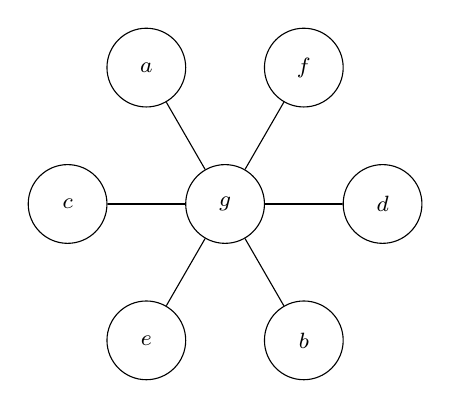
\begin{tikzpicture}[line cap=round, line join=round, >=stealth, font=\footnotesize, scale=1]
			\def\r{0.5cm}
			\draw (0,0) coordinate (g)  -- (0:2cm) coordinate (d) ;
			\draw (0,0) coordinate (g) -- (60:2cm) coordinate (f);	
			\draw (0,0) coordinate ( g)  -- (120:2cm) coordinate (a);	
			\draw (0,0) coordinate ( g)  -- (180:2cm) coordinate (c);
			\draw (0,0) coordinate ( g) -- (-120:2cm) coordinate (e);
			\draw (0,0) coordinate( g) -- (-60:2cm) coordinate (b);			
			\foreach \u in {g,d,f,a,c,e,b}{\filldraw[white] (\u) circle (\r);}
			\foreach \i in {g,d,f,a,c,e,b}{\draw (\i) circle (\r);\node at (\i) {$\i$};}
	\end{tikzpicture}}
	\par
	\shortans[0]{113}
	\loigiai{
		Số cách chọn $7$ số khác nhau từ tập $X$ là $\mathrm{C}_{14}^7$. Gọi $7$ số được chọn là $x_1 < x_2 < x_3 < x_4 < x_5 < x_6 < x_7$.\\
		Với mỗi tập hợp $7$ số được chọn, tổng số cách xếp vào $7$ ô tròn (do các vị trí là phân biệt) là $7!$.\\
		Ta sẽ đếm số cách xếp sao cho \textbf{không có hàng nào} được sắp xếp theo chiều tăng dần hoặc giảm dần (gọi là cách xếp \textit{lệch}).\\
		Một hàng (ví dụ gồm $3$ ô $a, g, b$) không tăng dần cũng không giảm dần khi và chỉ khi số ở ô trung tâm $g$ không nằm giữa hai số ở hai ô ngoài cùng. Nghĩa là $g$ phải lớn hơn cả hai số hoặc nhỏ hơn cả hai số ở hai đầu.\\
		Do đó, ở mỗi hàng, hai số ở hai đầu phải cùng lớn hơn $g$ hoặc cùng nhỏ hơn $g$. Vì có $3$ hàng nên tổng số lượng các số nhỏ hơn $g$ (trong $6$ số ở các ô bên ngoài) phải là một số chẵn. Các trường hợp có thể xảy ra:
		\begin{itemize}
			\item \textbf{Trường hợp 1:} Có $0$ số nhỏ hơn $g$. Khi đó $g = x_1$. Cả $6$ số còn lại đều lớn hơn $g$ nên xếp vào $6$ vị trí bên ngoài tùy ý đều thỏa mãn. Có $6!$ cách xếp.
			\item \textbf{Trường hợp 2:} Có $6$ số nhỏ hơn $g$. Khi đó $g = x_7$. Tương tự, có $6!$ cách xếp.
			\item \textbf{Trường hợp 3:} Có $2$ số nhỏ hơn $g$. Khi đó $g = x_3$. Hai số nhỏ hơn $g$ là $x_1$, $x_2$ bắt buộc phải nằm ở hai đầu của cùng một hàng.
			Ta chọn $1$ trong $3$ hàng để xếp $x_1$, $x_2$ (có $\mathrm{C}_3^1$ cách), hoán vị $x_1, x_2$ vào $2$ đầu hàng đó có $2!$ cách. Còn lại $4$ số lớn hơn $g$ xếp vào $4$ vị trí trống có $4!$ cách.
			Tổng số cách xếp ở trường hợp này là $\mathrm{C}_3^1 \cdot 2! \cdot 4!$.
			\item \textbf{Trường hợp 4:} Có $4$ số nhỏ hơn $g$. Khi đó $g = x_5$. Tương tự, có $2$ số lớn hơn $g$ là $x_6, x_7$ bắt buộc phải nằm ở hai đầu của cùng một hàng. Lập luận tương tự ta cũng có $\mathrm{C}_3^1 \cdot 2! \cdot 4!$ cách xếp.
		\end{itemize}
		Vậy số cách xếp \textit{lệch} đối với mỗi tập $7$ số được chọn là
		\[ 2 \cdot 6! + 2 \cdot \mathrm{C}_3^1 \cdot 2! \cdot 4! = 1\,440 + 288 = 1\,728 \text{ (cách)}. \]
		Số cách xếp thỏa mãn đề bài (có ít nhất một hàng tăng dần hoặc giảm dần) đối với mỗi tập $7$ số là
		\[ 7! - 1\,728 = 5\,040 - 1\,728 = 3\,312 \text{ (cách)}. \]
		Tổng số cách xếp thỏa mãn yêu cầu của toàn bộ bài toán là
		\[ T = \mathrm{C}_{14}^7 \cdot 3\,312 = 3\,432 \cdot 3\,312 = 11\,366\,784. \]
		Vậy ba chữ số có nghĩa đầu tiên của $T$ là $113$.
	}
\end{ex}
%%%=============================%%%
\Closesolutionfile{ans}
\newpage
\indapan{12}{ans/ansTN-Dung}
\indapan[TF]{2}{ans/ansTN-DungSai}
\indapan[SA]{6}{ans/ansTN-DienKhuyet}
%%%%%%%%%%%%%%
%%nhãn kết thúc đề (để đếm số trang tự động mỗi đề)
\label{B\thedeso}